\section{Cuantización y Despliegue}
\label{sec:quantization}

La etapa de despliegue convierte un checkpoint entrenado en un artefacto compacto mediante empaquetado ternario de pesos \citep{wang_bitnet_2023} y escalado de activaciones INT8, con estimaciones de tamaño alineadas con objetivos de despliegue ligero \citep{samson_lightweight_2026,bravin_embbert_2026}. El mismo subcomando emite artefactos estándar o cuantizados, o exporta formatos HuggingFace Transformers y BitNet GGUF para runtimes externos. Las formulaciones y las estimaciones de tamaño se remiten al Apéndice~\ref{sec:annex-norm-bitnet-mod}.

\begin{figure}[t]
\centering
\fitfigure{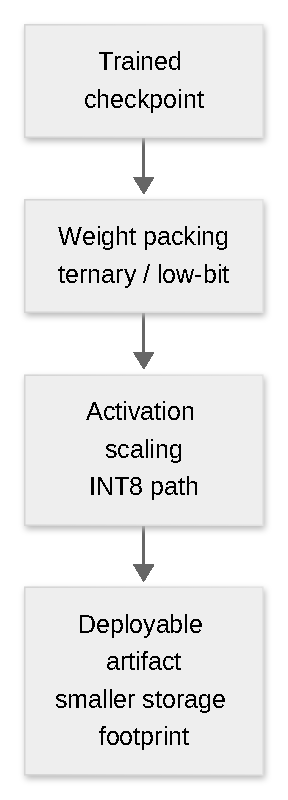
\includegraphics{../paper/figures/deploy-flow.pdf}}
\caption{Ruta de despliegue desde un checkpoint entrenado hasta un artefacto compacto. La cuantización es una transformación de la etapa de despliegue, no una familia de modelos separada.}
\label{fig:deploy-flow}
\end{figure}
